\section{VQA and QNN}
\begin{itemize}
    \item Basic concepts: \textbf{Cost function, ansatz, gradients, optimizers}
    \item Global and local cost function
    \item Some illustration?
\end{itemize}

Hybrid techniques involving Quantum circuits and Classical optimizers have been proposed to overcome the restrictions of Noisy Intermediate-Scale Quantum (NISQ) \cite{brooksQuantumSupremacyHunt2019} devices. 
Those constraints are the absence of fault-tolerant design, the limitation of qubit number per processor, and executable circuit depth. 
Moreover, quantum gates are static by design, which means every new data input to a quantum algorithm will produce a different quantum circuit.

Quantum circuits with trainable parameters can be created using Variational Quantum Algorithms (VQAs) \cite{cerezo2021variational}, which act as reusable circuit templates for quantum computers.
On the other hand, the classical optimizer perceives variational circuits as a black box that yields outputs from inputs and the trainable parameter.

Consider a simple problem that we want to solve using VQA, given the access to the training data.
The first step is to define a \textit{cost function} $C$ to search for a solution, we aim to minimize this cost function during the training process.
Then, we develop an \textit{ansatz}, this is the unitary operation that depends on a set of parameters $\theta$.
$\theta$ can be trained in a hybrid quantum-classical process to solve the problem.

\begin{figure}
    \centering
    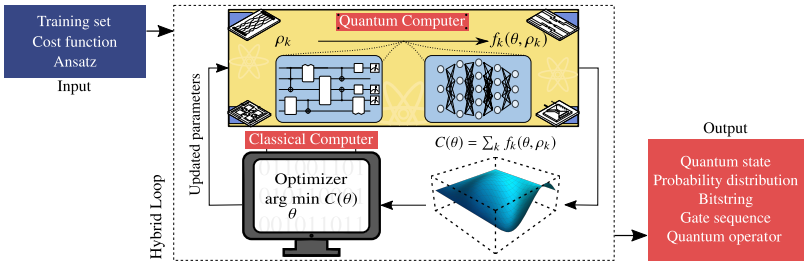
\includegraphics[width=\textwidth]{LiteratureReview/Appendices/vqadiagram.png}
    \caption{An illustrative diagram of VQA. The algorithm receives: a cost function $C(\theta)$ for $\theta$ is a set of parameters that encodes the solution; an ansatz is trained in the hybrid loop to solve the task; a set of training data ${\rho_k}$}
    \label{VQA diagram}
\end{figure}

\almarginpar{I thought the VQA and QNN reviews would be more extensive?}VQA is also the most widely used method for developing Quantum Neural Network (QNN) circuits. 
As a result, QNN inevitably inherited some of VQA's flaws.
Many Quantum Machine Learning models suffer from the unsolvability Barren Plateaus \cite{zhaoReviewQuantumNeural2021} that prevent the growth of circuit depth and lead the trainable parameters to a dead end.
When training a QNN framework with a large number of qubits, this phenomenon occurs; the objective function becomes flat, making it nearly impossible to estimate the gradient, \cite{mccleanBarrenPlateausQuantum2018, zhaoAnalyzingBarrenPlateau2021} causing inefficiency in circuit training. 

